\section{System Overview}
%\section{System Framework}
\label{sec-system}

\begin{figure}
\centering
\subfigure[{\scriptsize Framework}]{\label{fig:framework}
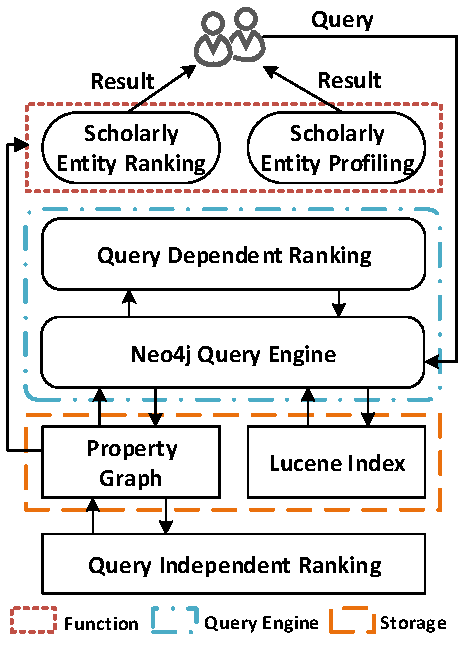
\includegraphics[width=0.4\columnwidth]{systemFrame.pdf}}
%\hspace{3ex}
\subfigure[{\scriptsize Neo4j schema}]{\label{fig:schema}
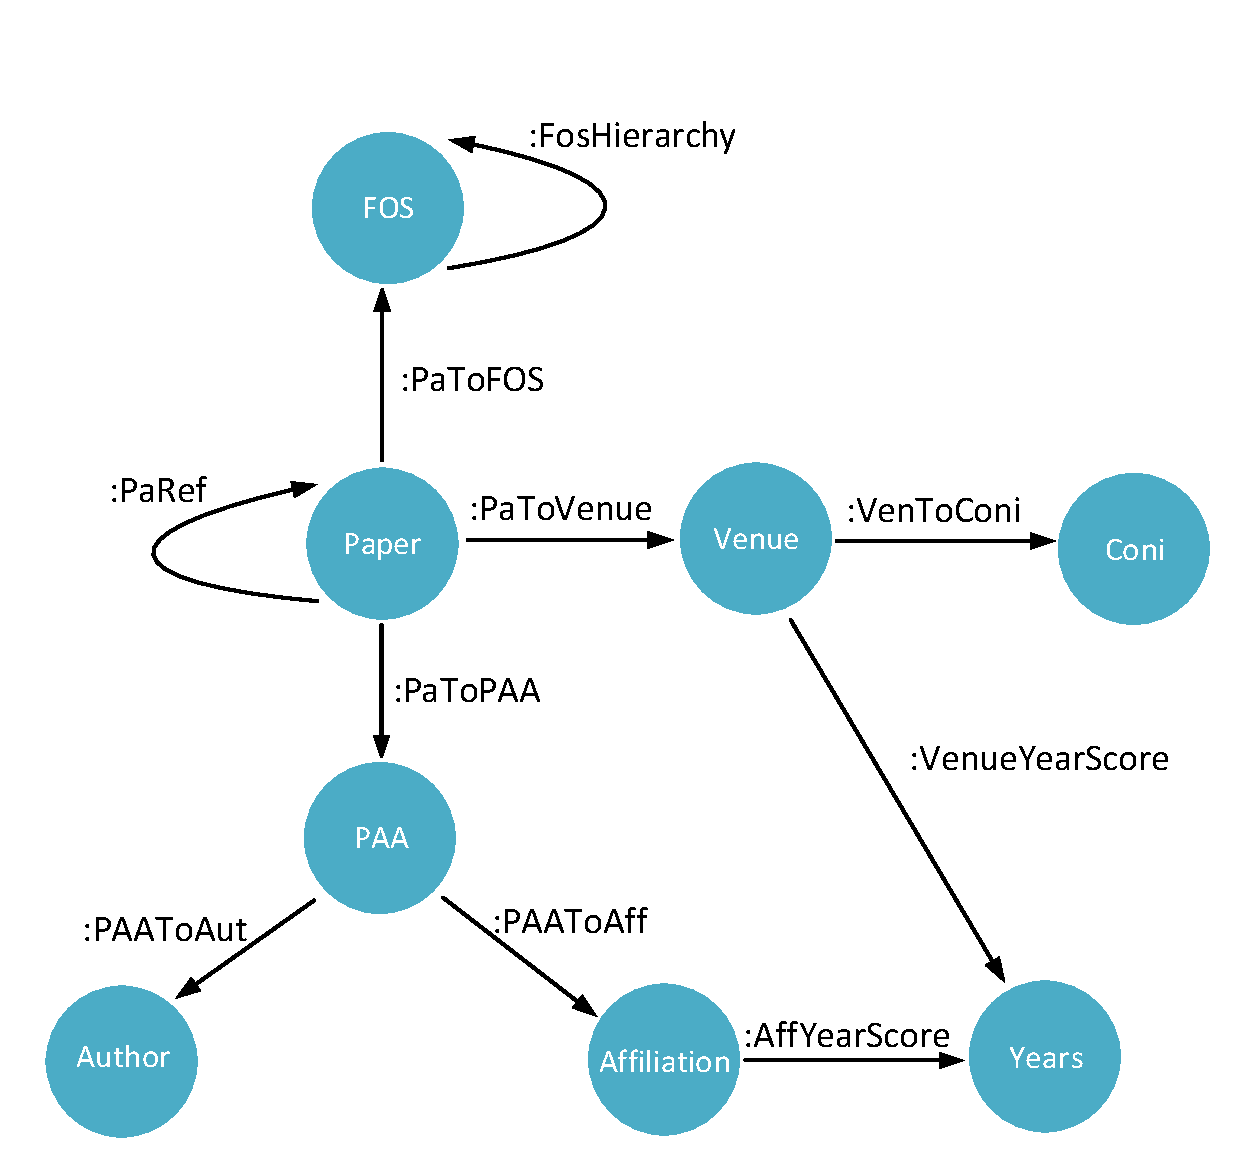
\includegraphics[width=0.56\columnwidth]{neo4jSchema.pdf}}
\caption{System design of \oursystem}
\label{fig:system}
%\vspace{-2ex}
\end{figure}


Figure \ref{fig:framework} shows the framework of our \oursystem. It consists of two main components, \ie \emph{Storage} and \emph{Query Engine}.
Below the storage component is a {\em Query-Independent Ranking} module that enriches the data with those pre-computed query-independent ranking scores. Note that there is another {\em Query-Dependent Ranking} module inside the query engine. Finally, two function modules on top present the analysis  to users based on the retrieved results. We next detail our system.

\subsection{Schema Design} \label{subsec:schema}

Graph database Neo4j is adopted for storage in \oursystem. As such, we need to design a schema that abstracts the entities and linked structures (\eg citation, authored-by).
% schema design rationaile
We follow two principles for schema design: (a) nodes for entities and relationships for linked structures, and (b) trading space for query efficiency if affordable and possible.

%reducing fine-grained relationship names while increase generic relationships qualified with property appropriately.

The schema is presented in Fig.~\ref{fig:schema}, where texts nears nodes and relationships represent properties of entities and linked structures, respectively.
It contains seven basic types of nodes including {\em Paper}, {\em Author}, {\em Affiliation}, {\em Venue}, {\em FOS} (field of study), {\em ConIns} (conferences instance in each year) and {\em Year}.
In addition, it further incorporates an artificial type of nodes, \ie {\em PAA} representing paper-author-affiliation tuples. Here we use extra space to improve query efficiency, \ie an author and her/his affiliation can be retrieved in one query.
%
Our schema also forms a total of nine types of relationships, one of which, \ie {\em :VenueScore}, has a weight property {\em score} and the rest are unweighted.
As another space-efficiency trade-off, those {\em Paper} nodes also use extra space on properties to maintain conference ID, journal ID and year.



\subsection{Graph Storage} \label{subsec:storage}

%Thus, we model scholarly data as a huge heterogeneous graph, shown in Fig. \ref{fig:schema}, which contains more than one billion nodes and over two billion relationships.
% 126909021 paper  114698044 articles 529 million, node:1032827519, relationship:1933421586

Based on the above schema, we store our scholarly data, \ie MAG~\cite{sinha2015overview}, as a huge property graph with more than 1.03 billion nodes and 1.93 billion relationships. We further clarify our graph storage with the following two points.

%Neo4j with native graph storage ensures that scholarly data is stored efficiently and relationships close to each other. We have proved through experiments that index-free adjacency is more efficient and cheaper, shown in Section~\ref{sec-demo}. Moreover, we highlight our graph storage on the following two points.
% neo4j native graph storage.

First, based on the original scholarly data, the {\em Query-Independent Ranking} module pre-computes those query-independent ranking metrics, \ie numbers of citations of papers, importance scores of papers, authors, venues and affiliations~\cite{ma2018query}. These scores are assigned as properties to the corresponding nodes.  
Note that iteratively accessing the linked entities is the most essential operation in the pre-computation. And it is much more convenient with graph storage.
Moreover, both citation numbers and importance scores support incremental computation~\cite{ma2018query} and are easier to dynamically maintain once the property graph gets updated.

%given that our query independent ranking, a type of Time-Weighted PageRank based on graph, assesses the importance of nodes in the heterogeneous scholarly graph. Thus, it is much more convenient to compute the importance score when employ graph storage. Secondly,
%we recompute the scholarly graph once scholarly data gets updated through incremental algorithm~\cite{ma2018query}. We can easily operate the affected areas of the scholarly graph on the graph storage. (weak? we do not implement in \oursystem) However, a huge volume index in RDBMS will cause significant performance bottleneck when update.
% benefits��PageRank algorithm. incremental computation. update index??? in neo4j and mysql. in stages

Second, to facilitate query processing on a billion-scale property graph, Lucene index is utilized for initial entity lookups. Specifically, we create fulltext indices for paper titles and affiliation names. These enable to efficiently find papers and affiliations whose titles and names contain a specific keyword. Besides, we also create schema indices for the entire author and venue names. %for efficient initial entity lookup.

%Other properties, such as {\em Author name} and {\em Paper ID}, are also created index for initial entity lookups.
% lucene index. Why we need lucene index. index what. result.
%  with IKAnalyzer to support Chinese

\eat{
\marked{highlight graph storage, query engine detail}

\marked{relation to ranking model, when to do ranking}

\marked{incremental computation}


(2) property graph (billion-scale) -- lucene index
%(1) adopt neo4j
%(2)

Storage is a key factor for the success of scholarly analysis systems, due to the large volume of scholarly data (\eg \oursystem mainly uses the MAG data with 126 and 529 million articles and citations, respectively~\cite{sinha2015overview}) and the complex entities and relationships.
%
Traditional RDBMS are used by CiteSeerx, AMiner and Semantic Scholar to manage scholarly data. On the other hand, Acemap and Microsoft Academic exploit distributed file systems.
%
We observe that entities in scholarly data are inherently linked. The existing storage solutions all ignore such linked feature, and may face challenges for efficient and high-concurrent query processing when the computing resources are limited. For instance, complex join operations in RDBMS will become the bottleneck when processing queries such as {\em finding all articles of someone's co-authors}.
%
To this end, we propose to utilize a popular graph database Neo4j to store and manage the large-scale, heterogeneous and linked scholarly data in \oursystem.
}

%Scholarly data highly connected by reference relationship between articles and constructs a huge heterogeneous graph.  Take RDBMS as an example, complex joins and self-joins will incur obviously performance bottleneck when the scholarly dataset becomes more inter-related. A comparison of the performance of querying the cited articles of an article using RDBMS(Mysql) and graph database(Neo4j) is given in table 1. Furthermore, our heterogeneous entities ranking algorithm, a type of Time-Weighted PageRank bases on graph structure, assesses the importance of nodes in a heterogeneous graph. Thus, it utilizes a popular graph database Neo4j to store and manage heterogeneous scholarly data.
% scholarly data source, currently solution, why graph database.

%Intuitively, a paper get published in a journal/conference by the author means new edges among paper, author and venue node. By employing ranking model as stated in section \ref{sec-model}, we derive affiliation, author, venue and article ranking score using incremental computation \cite{ma2018query}. And those score is described as a property in the graph schema.
% explain our schema



% design principles and schema.
% We take into consideration of the query ability of the graph schema and adopt specific time and space trade-offs. heterogeneous scholarly entity ranking ?

%In fact, we can apply any other ranking algorithms to rank scholarly entities in the graph schema.



\begin{figure}
\centering
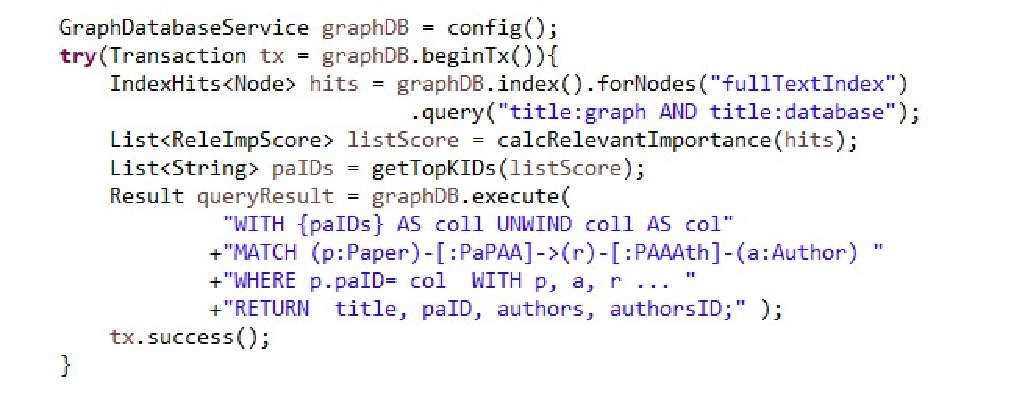
\includegraphics[width=\columnwidth]{queryProcess.pdf}
\caption{An example workflow of the query engine}
\label{fig:queryProcess}
%\vspace{-3ex}
\end{figure}

\subsection{Graph Query Engine} \label{subsec:qe}
\oursystem supports a variety of graph queries on the property graph. And the {\em Query Engine} is responsible for processing this set of queries. When a query is issued, {\em Neo4j Query Engine} first translates it into a cypher with proper parsing and semantic analysis.
Note that, when applicable, the cypher is revised by hitting the Lucene index and directly using the returned entity IDs. Rankings given by the {\em Query-Dependent Ranking} module, \ie relevance and relevant importance-based rankings may also be included in the cypher if needed. Based on the final cypher, an optimized query plan is generated and processed on the property graph.


Figure~\ref{fig:queryProcess} gives an example workflow of the query engine that users want to retrieve the top scholarly articles about ``graph database"  ranked by relevant importance. The fulltext index is firstly hit to get the related paper IDs on ``graph database'' (lines 4--5). The {\em Query-Dependent Ranking} module then calculates the relevant importance scores of those related papers and the top-k paper IDs are further identified (lines 7--8). Based on the complete cypher, the {\em Neo4j Query Engine} finally generates the query plan, executes it on the property graph and gets the results (lines 10--15).

\subsection{Function Modules}
Finally, the two function modules on top collect the scholarly entities ranked and returned from the back-end, and present some (visual) analysis to users. Moreover specifically, \oursystem utilizes RESTful APIs  and Echarts\footnote{http://echarts.baidu.com/} to display the scholarly ranking and profiling results. Detailed demonstrations are available in next section.


% visualization do what ?
% restful API
% scenarios, Query and Ranking Scholarly Entity, Author Profiling.
%Based on the graph storage, scholarly data was managed and processed in the system back-end. \oursystem collects user querys, dispatch to query engine and the results are then presented by visualizer using RESTful API. We employ Echarts (http://echarts.baidu.com/) to display scholarly article analysis and author profiling, detailed demonstrations are accessed in next section.
% function implement in back-end, echarts js  using RESTful API. demonstrate xxx in the next section.


%With scholarly data management and processing in the system back-end, the visualizer of \oursystem collects user queries through user interfaces. The queries are to the query engine and the returned results are then presented by visualizer. We will demonstrate some scholarly analysis scenarios in the next Section.


%\begin{table}[t!]
%%\begin{center}
%\caption{Query TopK Articles by Relevant Importance }
%\label{tab-codeExample}
%\begin{scriptsize}
%\begin{tabular}{ l}
%\hline
%{An Example procedure of Query TopK Articles by Relevant Importance } \\
%\hline
%1. GraphDatabaseService graphDB = new GraphDatabaseFactory()... ; \\
%2.  \hspace{6ex}  try(Transaction tx = graphDB.beginTx()) \{ \\
%3.  \hspace{12ex} 	IndexHits $\langle$ Node$\rangle$ hits = db.index().forNodes("fulltext") \\
%    \hspace{20ex}   .query("titile: graph AND title:database"); \\
%4.  \hspace{12ex} 	List$\langle$ ReleImpScore$\rangle$ listScore = calcRelevantImportance(hits); \\
%5.  \hspace{12ex} 	List$\langle$ String$\rangle$  paIDs = getTopKIDs(listScore); \\
%6.  \hspace{12ex}    Result result = graphDB.execute(`` \\
%    \hspace{20ex}		WITH \{paIDs\} AS coll UNWIND coll AS col \\
%    \hspace{20ex}		MATCH (p:Paper)-[:PaToPAA]-$>$(r)-[:PAAToAut]-(a:Author)\\
%	\hspace{20ex}		WHERE p.paID= col  WITH p, r, a, ... \\
%	\hspace{20ex}		RETURN  title, paID, authors, authorsID; ");\\
%7.	\hspace{12ex}	tx.success();\\
%    \hspace{6ex}  \} \\
%\hline
%\end{tabular} \\ %\vspace{.5ex}
%\end{scriptsize}
%%\end{center}
%\end{table}

